\chapter{进程与异常}

\section{实验目的}
  \begin{enumerate}
    \item 创建一个进程并成功运行
    \item 实现时钟中断,通过时钟中断内核可以再次获得执行权
    \item 实现进程调度,创建两个进程,并且通过时钟中断切换进程执行
  \end{enumerate}

在本次实验中你将运行一个用户模式的进程。你需要使用数据结构进程控制块 Env 来跟踪用户进程。
通过建立一个简单的用户进程,加载一个程序镜像到进程控制块中,并让它运行起来。
同时,你的MIPS内核将拥有处理异常的能力。

\section{进程}

\begin{note}
进程既是基本的分配单元,也是基本的执行单元。第一,进程是一个实体。每一个进程都有它自己的地址空间,
一般情况下,包括代码段、数据段和堆栈。第二,进程是一个“执行中的程序”。
程序是一个没有生命的实体,只有处理器赋予程序生命时,它才能成为一个活动的实体,我们称其为进程。
\end{note}

\subsection{进程控制块}

这次实验是关于进程和异常的,那么我们首先来结合代码看看进程控制块是个什么东西。

进程控制块(PCB)是系统为了管理进程设置的一个专门的数据结构,用它来记录进程的外部特征,描述进程的运动变化过程。
系统利用PCB来控制和管理进程,所以\textbf{PCB是系统感知进程存在的唯一标志。进程与PCB是一一对应的。}
通常PCB应包含如下一些信息:

\begin{codeBoxWithCaption}{进程控制块\label{code:process_of_env.h}}
  \inputminted[linenos]{c}{codes/process_of_env.h}
\end{codeBoxWithCaption}

为了集中你的注意力在关键的地方,我们暂时不介绍其他实验所需介绍的内容。
下面是\textbf{lab3}中需要用到的这些域的一些简单说明:

\begin{itemize}
  \item env\_tf : Trapframe 结构体的定义在\textbf{include/trap.h} 中,env\_tf 的作用就是在进程因为时间片用光不再运行时,将其当时的进程上下文环境保存在env\_tf 变量中。当从用户模式切换到内核模式时,内核也会保存进程上下文,因此进程返回时上下文可以从中恢复。
  \item env\_link : env\_link 的机制类似于实验二中的 pp\_link,使用它和 env\_free\_list 来构造空闲进程链表。
  \item env\_id : 每个进程的 env\_id 都不一样,env\_id 是进程独一无二的标识符。
  \item env\_parent\_id : 该变量存储了创建本进程的进程 id。
  这样进程之间通过父子进程之间的关联可以形成一颗进程树。
  \item env\_status : 该变量只能在以下三个值中进行取值:
  \begin{itemize}
    \item ENV\_FREE : 表明该进程是不活动的,即该进程控制块处于进程空闲链表中。
    \item ENV\_NOT\_RUNNABLE : 表明该进程处于阻塞状态,
    处于该状态的进程往往在等待一定的条件才可以变为就绪状态从而被CPU调度。
    \item ENV\_RUNNABLE : 表明该进程处于就绪状态,正在等待被调度,
    但处于RUNNABLE状态的进程可以是正在运行的,也可能不在运行中。
  \end{itemize}
  \item env\_pgdir : 这个变量保存了该进程页目录的虚拟地址。
  \item env\_cr3 : 这个变量保存了该进程页目录的物理地址。
\end{itemize}

这里值得强调的一点就是\textbf{ENV\_RUNNABLE 状态并不代表进程一定在运行中,它也可能正处于调度队列中}。
而我们的进程调度也只会调度处于RUNNABLE状态的进程。

既然我们知道了进程控制块,我们就来认识一下进程控制块数组\textbf{envs}。在我们的实验中,
存放进程控制块的物理内存在系统启动后就要被分配好,并且这块内存不可被换出。
所以需要在系统启动后就要为envs数组分配内存,下面你就要完成这个重任

\begin{exercise}
  \begin{itemize}
    \item 修改pmap.c/mips\_vm\_init函数来为envs数组分配空间。
    \item envs数组包含 NENV 个Env结构体成员,你可以参考pmap.c中已经写过的\textbf{pages}数组空间的分配方式。
    \item 除了要为数组 envs 分配空间外,你还需要使用 pmap.c 中你填写过的一个内核态函数为其进行段映射,
    envs 数组应该被\textbf{UENVS}区域映射,你可以参考\textbf{./include/mmu.h}。	
  \end{itemize}
\end{exercise}

当然我们光有了存储进程控制块信息的envs还不够,我们还需要像lab2一样将空闲的env控制块按照链表形式“串”起来,便于后续分配ENV结构体对象,形成env\_free\_list。一开始我们的所有进程控制块都是空闲的,所以我们要把它们都“串”到env\_free\_list上去。

\begin{exercise}
仔细阅读注释,填写\textbf{env\_init}函数,注意要按照逆序插入(函数位于lib/env.c中)。
\end{exercise}

在填写完env\_init函数后,我们对于envs的操作暂时就告一段落了,不过我们还有一个小问题没解决,注释里说明了要逆序插入,但是为什么呢?我们需要你来仔细思考,注释中已经给出了提示。

\begin{thinking}\label{think-env_init}
为什么我们在构造空闲进程链表时使用了逆序插入的方式?
\end{thinking}

\subsection{设置进程控制块}

做完上面那个小练习后,那么我们就可以开始利用\textbf{空闲进程链表env\_free\_list}创建进程来玩了。下面我们就来具体讲讲你应该如何创建一个进程\footnote{这里我们创建进程是指系统创建进程,不是指fork等进程“生”进程。我们将在lab4中接触另一种进程创建的方式。}。

进程创建的流程如下:

\begin{description}
  \item[第一步] 申请一个空闲的PCB,从env\_free\_list中索取一个空闲PCB块,这时候的PCB就像张白纸一样。
  \item[第二步] “纯手工打造”打造一个进程。在这种创建方式下,由于没有模板进程,所以进程拥有的所有信息都是手工设置的。
  而进程的信息又都存放于进程控制块中,所以我们需要手工初始化进程控制块。
  \item[第三步] 进程光有PCB的信息还没法跑起来,每个进程都有独立的地址空间。\label{process-3}
  所以,我们要为新进程分配资源,为新进程的程序和数据以及用户栈分配必要的内存空间。
  \item[第四步] 此时PCB已经被涂涂画画了很多东西,不再是一张白纸,把它从空闲链表里除名,就可以投入使用了。
\end{description}

当然,第二步的信息设置是本次实验的关键,那么下面让我们来结合注释看看这段代码

\begin{codeBoxWithCaption}{进程创建\label{code:env_alloc.c}}
  \inputminted[linenos]{c}{codes/env_alloc.c}
\end{codeBoxWithCaption}

相信你一眼看到第三条注释的时候一定会吐槽:“什么鬼,什么叫合适的值啊”。淡定,先别着急吐槽,先花半分钟的时间看一下第二条注释。

下面这个函数就是你在第二步中要使用的函数。在用之前,我们希望你仔细看注释,并对这个函数进行一些思考。

\begin{codeBoxWithCaption}{地址空间初始化\label{code:env_setup_vm.c}}
  \inputminted[linenos]{c}{codes/env_setup_vm.c}
\end{codeBoxWithCaption}

请在仔细看完上述函数的注释和其中的Hint后,来思考一下下面这些为你准备的问题

\begin{thinking}\label{think-env_setup_vm}
思考env\_ setup\_ vm函数:
\begin{itemize}
\item 第三点注释中的问题:为什么我们要执行\mintinline{c}|pgdir[i] = boot_pgdir[i]|这个赋值操作?换种说法,我们为什么要使用\mintinline{c}|boot_pgdir|作为一部分模板?(提示:mips虚拟空间布局)
\item {\small UTOP}和{\small ULIM}的含义分别是什么,在{\small UTOP}到{\small ULIM}的区域与其他用户区相比有什么最大的区别?
\item (选做)我们为什么要让\mintinline{c}|pgdir[PDX(UVPT)]=env_cr3?|(提示:结合系统自映射机制)
\end{itemize}
\end{thinking}

其实第三点注释问题本身要思考起来是有比较大跨度的,所以我们直接在这里给出笔者在反复思考与理解后所获得的心得,
鼓励你在写文档时可以进行更多思考与更深层的理解:)。

在我们的实验中,对于不同的进程而言,虚拟地址ULIM以上的地方,虚拟地址到物理地址的映射关系都是一样的。
因为这2G虚拟空间,不是由哪个进程管理的,而是由内核管理的!如果你仔细思索这句话,
可能会产生疑惑:“那为什么不能该内核管的时候让内核进程去管,该普通进程管的时候给普通进程去管,
非要混在一个地址空间里搞来搞去的呢?”这种想法是很好的,但是问题来了,在我们这种布局模式下,
有严格意义上的内核进程吗?

答案当然是否定的,这里我们要再讲清楚几个概念,方可解决这个问题。

首先来科普下虚拟空间的分配模式。我们知道,每一个进程都有4G的逻辑地址可以访问,
我们所熟知的系统不管是Linux还是Windows系统,都可以支持3G/1G模式或者2G/2G模式。
3G/1G模式即满32位的进程地址空间中,用户态占3G,内核态占1G。这些情况在进入内核态的时候叫做陷入内核,
因为\textbf{即使进入了内核态,还处在同一个地址空间中,并不切换CR3寄存器。}
但是!还有一种模式是4G/4G模式,内核单独占有一个4G的地址空间,所有的用户进程独享自己的4G地址空间,
这种模式下,在进入内核态的时候,叫做切换到内核,\textbf{因为需要切换CR3寄存器},
所以进入了\textbf{不同的地址空间}!

\begin{note}
用户态和内核态的概念相信大家也不陌生,内核态即计组实验中所提到的特权态,用户态就是非特权态。
mips汇编中使用一些特权指令如\mintinline{gas}|mtc0|、\mintinline{gas}|mfc0|、\mintinline{gas}|syscall|等都会陷入特权态(内核态)。
\end{note}

而我们这次实验,根据\mintinline{c}|./include/mmu.h|里面的布局来说,我们是2G/2G模式,
用户态占用2G,内核态占用2G。接下来,也是最容易产生混淆的地方,进程从用户态提升到内核态的过程,
操作系统中发生了什么?

是从当前进程切换成一个所谓的“内核进程”来管理一切了吗?不!还是一样的配方,还是一样的进程!
改变的其实只是进程的权限!我们打一个比方,你所在的班级里没有班长,
任何人都可以以合理的理由到老师那申请当临时班长。你是班里的成员吗?当然是的。
某天你申请当临时班长,申请成功了,那么现在你还是班里的成员吗?当然还是的。
那么你前后有什么区别呢?是权限的变化。可能你之前和其他成员是完全平等,互不干涉的。
那么现在你可以根据花名册点名,你可以安排班里的成员做些事情,你可以开班长会议等等。
那么我们能说你是班长吗?不能,因为你并不是永久的班长。但能说你拥有成为班长的资格吗?
当然可以,这种\textbf{成为临时班长的资格},我们可以粗略地认为它就是内核态的精髓所在。

而在操作系统中,每个完整的进程都拥有这种成为临时内核的资格,即所有的进程都可以发出申请变成内核态下运行的进程。
内核态下进程可访问的资源更多,更加自由。在之后我们会提到一种“申请”的方式,就叫做“系统调用”。

那么你现在应该能够理解为什么我们要将内核才能使用的虚页表为每个进程都拷贝一份了,在2G/2G这种布局模式下,
每个进程都会有\textbf{2G内核态}的虚拟地址,以便临时变身为“内核”行使大权。但是,在变身器使用之前,就算是奥特曼,
一样也只能访问自己的那2G用户态的虚拟地址。

那么这种微妙的关系应该类似于下面这种:(图中灰色代表不可用,白色代表可用)
\begin{figure}[htbp]
  \centering
  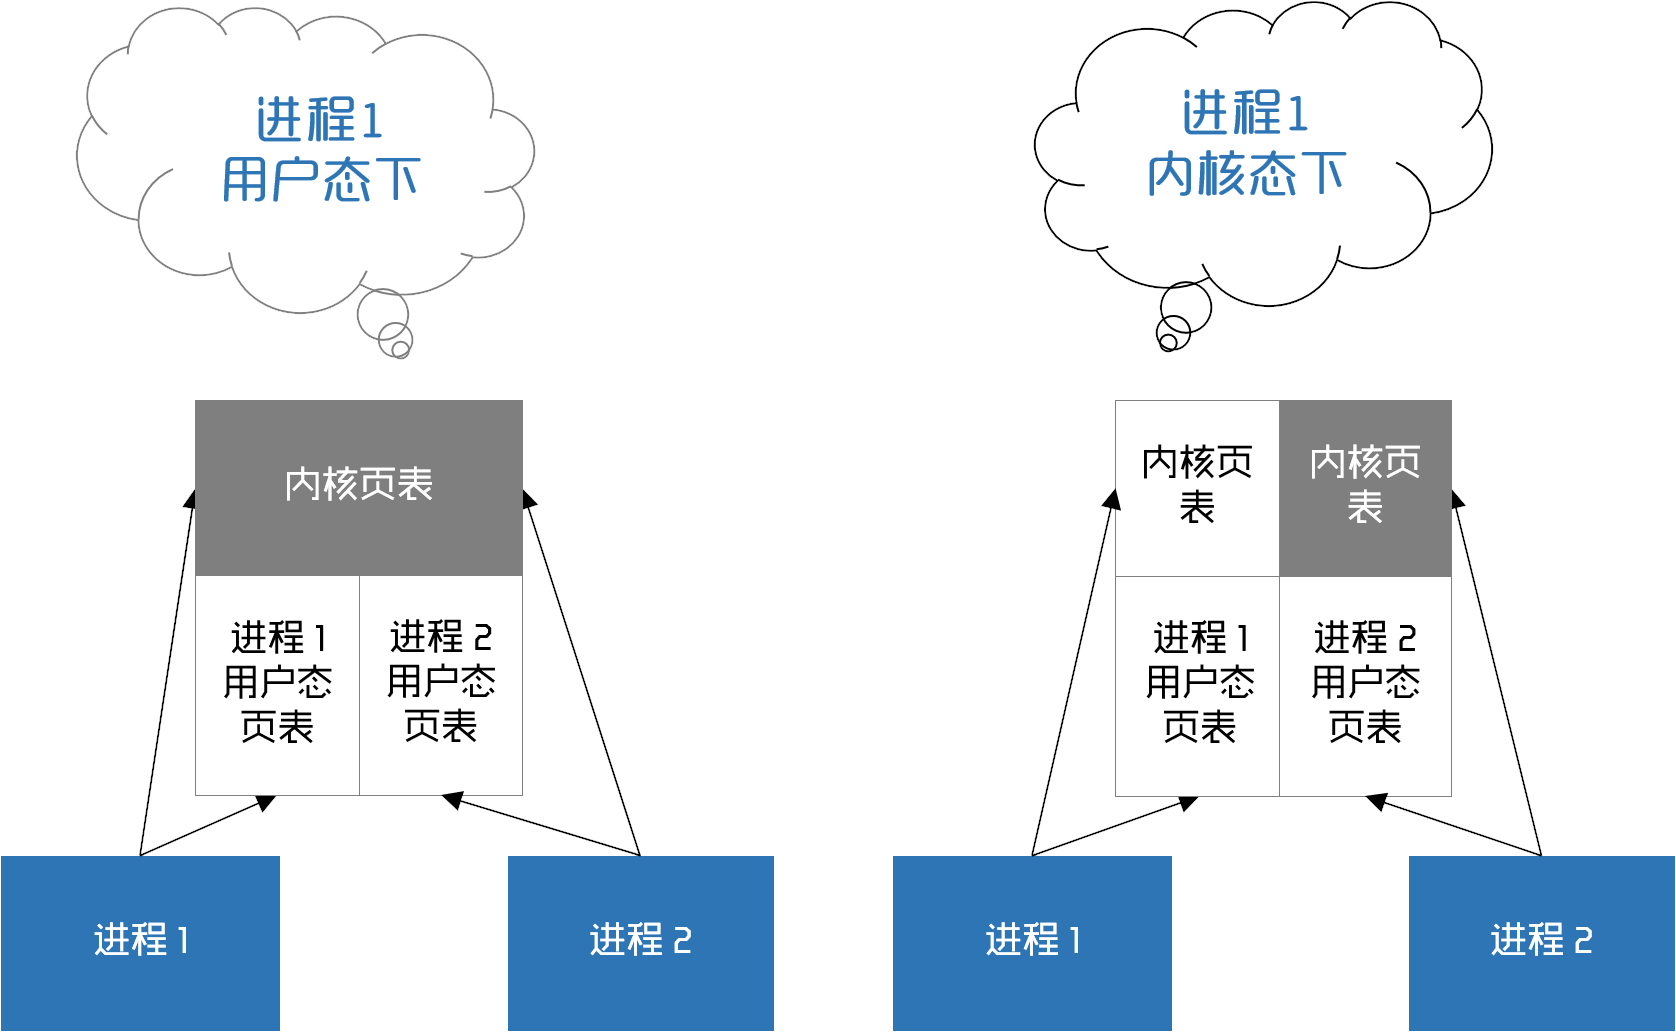
\includegraphics[width=14cm]{Process}
  \caption{进程页表与内核页表的关系}\label{fig:Process} 
\end{figure}


在上述的思考完成后,那么我们就可以直接在\textbf{env\_alloc} 第二步直接使用该函数了。
现在来解决一下刚才的问题,第三点所说的合适的值是什么?我们要设定哪些变量的值呢?

我们要设定的变量其实在\textbf{env\_alloc} 函数的提示中已经说的很清楚了,至于其合适的值,
相信仔细的你从函数的前面长长的注释里一定能获得足够的信息。当然我要讲的重点不在这里,
重点在我们已经给出的这个设置\mintinline{c}|e->env_tf.cp0_status = 0x10001004;|

这个设置很重要,很重要,很重要,重要到我们必须直接在代码中给出。为什么说它重要,各位看官且听我娓娓道来。

\begin{figure}[htbp]
  \centering
  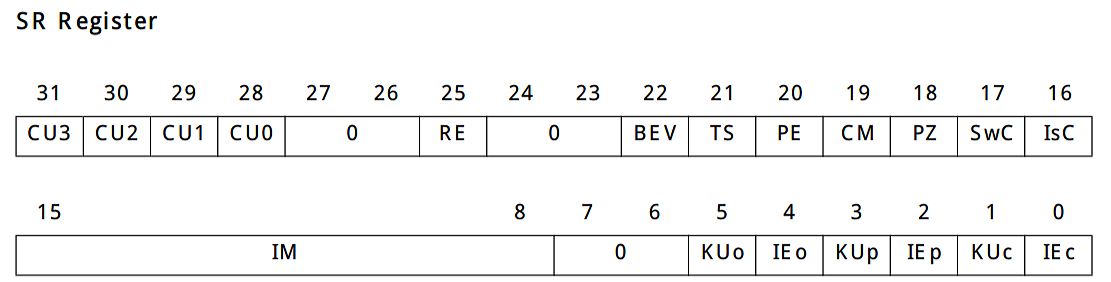
\includegraphics[width=15cm]{3-R3000_SR}
  \caption{R3000的SR寄存器示意图}\label{fig:3-R3000_SR} 
\end{figure}

图\ref{fig:3-R3000_SR}是我们MIPSR3000里的SR(status register)寄存器示意图,就是我们在env\_tf里的cp0\_ status。

第28bit设置为1,表示处于用户模式下。

第12bit设置为1,表示4号中断可以被响应。

这些都是小case,下面讲的才是重点!

R3000的SR寄存器的低六位是一个二重栈的结构。
KUo和IEo是一组,每当中断发生的时候,硬件自动会将KUp和IEp的数值拷贝到这里;
KUp和IEp是一组,当中断发生的时候,硬件会把KUc和IEc的数值拷贝到这里。

其中KU表示是否位于内核模式下,为1表示位于内核模式下;
IE表示中断是否开启,为1表示开启,否则不开启\footnote{我们的实验是不支持中断嵌套的,
所以内核态时是不可以开启中断的。}。

而每当rfe指令调用的时候,就会进行上面操作的\textbf{逆操作}。
我们现在先不管为何,但是已经知道,下面这一段代码在\textbf{运行第一个进程前是一定要执行的},
\label{env_pop_tf}所以就一定会执行\mintinline{gas}|rfe|这条指令。

\begin{minted}[linenos]{gas}
lw   k0,TF_STATUS(k0)        #恢复CP0_STATUS寄存器    
mtc0 k0,CP0_STATUS
j    k1
rfe
\end{minted}

现在你可能就懂了为何我们status后六位是设置为\mintinline{c}|000100b|了。
当运行第一个进程前,运行上述代码到\mintinline{gas}|rfe|的时候,就会将KUp和IEp拷贝回KUc和IEc,令status为 
\mintinline{c}|000001b|,最后两位KUc,IEc为\textbf{[0,1]},表示开启了中断。之后第一个进程成功运行,
这时操作系统也可以正常响应中断,Nice!

\begin{note}
{\small 关于MIPSR3000版本SR寄存器功能的英文原文描述:
The status register is one of the more important registers. The register has several
fields. The current Kernel/User (KUc) flag states whether the CPU is in kernel mode.
The current Interrupt Enable (IEc) flag states whether external interrupts are turned on.
If cleared then external interrupts are ignored until the flag is set again. In an exception
these flags are copied to previous Kernel/User and Interrupt Enable (KUp and IEp) and
then cleared so the system moves to a kernel mode with external interrupts disabled.
The Return From Exception instruction writes the previous flags to the current flags.}
\end{note}

当然我们从注释也能看出,第四步除了需要设置\mintinline{c}|cp0status|以外,还需要设置栈指针。
在MIPS中,栈寄存器是第29号寄存器,注意这里的栈是用户栈,不是内核栈。

\begin{exercise}
根据上面的提示与代码注释,填写 \textbf{env\_ alloc} 函数。
\end{exercise}

%好,填到这里你可能有些疲倦了,我们来讲个笑话。

%\begin{note}
%从前有一个年轻人,他小时候就表示他渴望将来能成为一个伟大的作家。当被问及怎样才算是“伟大”时,
%他说:“我要写出全世界的人都会阅读的作品,这些作品会唤起人们内心最深处的情感,
%这些作品会让他们在痛苦和愤怒之中尖叫、哭泣和咆哮!”

%此人目前就职于微软公司,负责撰写错误信息。
%\end{note}

\subsection{加载二进制镜像}
%开心一笑过后,
我们继续来完成我们的实验。下面这个函数还是蛮难填的呢,所以大家一定要跟紧我的步伐,我们慢慢来分析一下这个函数。

我们在\hyperref[process-3]{进程创建}第三点曾提到过,我们需要为\textbf{新进程的程序}分配空间来容纳程序代码。
那么下面我需要有两个函数来一起完成这个任务

\begin{codeBoxWithCaption}{加载镜像映射\label{code:load_icode_mapper.c}}
  \inputminted[linenos]{c}{codes/load_icode_mapper.c}
\end{codeBoxWithCaption}

为了完成这个函数,我们接下来再补充一点关于ELF的知识。

前面在讲解内核加载的时候,我们曾简要说明过ELF的加载过程。这里,我们再做一些补充说明。要想正确加载一个ELF文件到内存,
只需将ELF文件中所有需要加载的segment加载到对应的虚地址上即可。为了降低难度,我们已经写好了用于解析ELF文件的代码
(lib/kernel\_elfloader.c),你可以直接调用相应函数获取ELF文件的各项信息,并完成加载过程。该函数的原型如下:

\begin{minted}[linenos]{c}
// binary为整个待加载的ELF文件。size为该ELF文件的大小。
// entry_point是一个u_long变量的地址(相当于引用),解析出的入口地址会被存入到该位置
int load_elf(u_char *binary, int size, u_long *entry_point, void *user_data,
             int (*map)(u_long va, u_int32_t sgsize,
                        u_char *bin, u_int32_t bin_size, void *user_data))
\end{minted}

我们来着重解释一下load\_elf()函数的设计,以及最后两个参数的作用。为了让你有机会完成加载可执行文件到内存的过程,
load\_elf()函数只完成了解析ELF文件的部分,而把将ELF文件的各个segment加载到内存的工作留给了你。
为了达到这一目标,load\_elf()的最后两个参数用于接受一个你的自定义函数以及你想传递给你的自定义函数的额外参数。
每当load\_elf()函数解析到一个需要加载的segment,会将ELF文件里与加载有关的信息作为参数传递给你的自定义函数。
你的自定义函数完成加载单个segment的过程。

为了进一步简化你的理解难度,我们已经为你定义好了这个“自定义函数”的框架。如代码\ref{code:load_icode_mapper.c}所示。
load\_elf()函数会从ELF文件文件中解析出每个segment的四个信息:va(该段需要被加载到的虚地址)、sgsize(该段在内存中的大小)、
bin(该段在ELF文件中的内容)、bin\_size(该段在文件中的大小),并将这些信息传给我们的“自定义函数”。

接下来,你只需要完成以下两个步骤:

\begin{description}
  \item[第一步] 加载该段在ELF文件中的所有内容到内存。
  \item[第二步] 如果该段在文件中的内容的大小达不到该段在内存中所应有的大小,那么余下的部分用0来填充。
\end{description}

也许机灵的你发现了一个很无语的情况:我们并没有真正解释清楚user\_data这个参数的作用。最后一个参数是一个函数指针,
用于将我们的自定义函数传入进去。但这个诡异的user\_data到底是做什么用的呢?这样设计又是为了什么呢?
很不幸,这个问题我们决定留给你来思考。

\begin{thinking}\label{think-user-data}
思考user\_data这个参数的作用。没有这个参数可不可以?为什么?(如果你能说明哪些应用场景中可能会应用这种设计就更好了。
可以举一个实际的库中的例子)
\end{thinking}

思考完这一点,我们就可以进入这一小节的练习部分了。

\begin{exercise}
通过上面补充的知识与注释,填充 \textbf{load\_ icode\_ mapper} 函数。
\end{exercise}

现在我们已经完成了补充部分最难的一个函数,那么下面我们完成这个函数后,
就能真正实现把二进制镜像加载进内存的任务了。

\begin{codeBoxWithCaption}{完整加载镜像\label{code:load_icode.c}}
  \inputminted[linenos]{c}{codes/load_icode.c}
\end{codeBoxWithCaption}

现在我们来根据注释一步一步完成这个函数。
在第二步我们要用第一步申请的页面来初始化一个进程的栈,根据注释你应当可以轻松完成。
这里我们只讲第三步的注释所代表的内容,其余你可以根据注释中的提示来完成。

第三步通过调用我们预先为你准备好的load\_elf()函数来将ELF文件真正加载到内存中。
这里仅做一点提醒:请将load\_icode\_mapper()这个函数作为参数传入到load\_elf()中。
其余的参数在前面已经解释过了,就不再赘述了。

\begin{exercise}
通过补充的ELF知识与注释,填充 \textbf{load\_ icode} 函数。
\end{exercise}

这里的\mintinline{c}|e->env_tf.pc|是什么呢?就是在我们计组中反复强调的甚为重要的\mintinline{c}|PC|。
它指示着进程当前指令所处的位置。你应该知道,冯诺依曼体系结构的一大特点就是
:程序预存储,计算机自动执行。我们要运行的进程的代码段预先被载入到了\textbf{entry\_ point}为起点的
内存中,当我们运行进程时,CPU将自动从pc所指的位置开始执行二进制码。

\begin{thinking}\label{think-位置}
思考上面这一段话,并根据自己在\textbf{lab2}中的理解,回答:
  \begin{itemize}
  \item 我们这里出现的"指令位置"的概念,你认为该概念是针对虚拟空间,还是物理内存所定义的呢?
  \item 你觉得\mintinline{c}|entry_point|其值对于每个进程是否一样?该如何理解这种统一或不同?
  \item 从布局图中找到你认为最有可能是\mintinline{c}|entry_point|的值。
  \end{itemize}
\end{thinking}

思考完这一点后,下面我们来准备准备可以真正创建进程了。

\subsection{创建进程}

创建进程的过程很简单,就是实现对上述个别函数的封装,\textbf{分配一个新的Env结构体,设置进程控制块,并将二进制代码载入到对应地址空间}即可完成。好好思考上面的函数,我们需要用到哪些函数来做这几件事?

\begin{exercise}
根据提示,完成 \textbf{env\_create} 函数的填写。
\end{exercise}

当然提到创建进程,我们还需要提到一个封装好的宏命令

\begin{minted}[linenos]{c}
#define ENV_CREATE(x) \
{ \
    extern u_char binary_##x##_start[];\
    extern u_int binary_##x##_size; \
    env_create(binary_##x##_start, \
        (u_int)binary_##x##_size); \
}
\end{minted}

这个宏里的语法大家可能以前没有见过,这里解释一下\mintinline{c}|##|代表拼接,例如\footnote{这个例子是转载的,出处为\url{http://www.cnblogs.com/hnrainll/archive/2012/08/15/2640558.html},想深入了解的同学可以参考这篇博客}

\begin{minted}[linenos]{c}
#define CONS(a,b) int(a##e##b) 
int main() 
{
    printf("%d\n", CONS(2,3));  // 2e3 输出:2000 
    return 0; 
}
\end{minted}

好,那么现在我们就得手工在我们的\mintinline{c}|init/init.c|里面加两句话来初始化创建两个进程

\begin{minted}[linenos]{c}
ENV_CREATE(user_A);
ENV_CREATE(user_B);
\end{minted}

这两句话加在哪里呢?那就需要你翻代码来寻找啦~

\begin{exercise}
根据注释与理解,将上述两条进程创建命令加入 \textbf{init/init.c} 中。
\end{exercise}

做完这些,是不是迫不及待地想要跑个进程看看能否成功?等我们完成下面这个函数,就可以开始第一部分的自我测试了!

\subsection{进程运行与切换}

\begin{codeBoxWithCaption}{进程的运行\label{code:env_run.c}}
  \inputminted[linenos]{c}{codes/env_run.c}
\end{codeBoxWithCaption}

刚刚说到的load\_icode 是为数不多的坑函数之一,env\_run 也是,而且其实按程度来讲可能更甚一筹。

env\_run,是进程运行使用的基本函数,它包括两部分:
\begin{itemize}
  \item 一部分是保存当前进程上下文(\textbf{如果当前没有运行的进程就跳过这一步})
  \item 另一部分就是恢复要启动的进程的上下文,然后运行该进程。
\end{itemize}

\begin{note}
进程上下文说来就是一个环境,相对于进程而言,就是进程执行时的环境。具体来说就是各个变量和数据,包括所有的寄存器变量、内存信息等。
\end{note}

其实我们这里运行一个新进程往往意味着是进程切换,而不是单纯的进程运行。进程切换,
人如其名,就是当前进程停下工作,让出CPU处理器来运行另外的进程。
那么要理解进程切换,我们就要知道进程切换时系统需要做些什么。Alt+Tab可以吗?当然不可以。
实际上进程切换的时候,为了保证下一次进入这个进程的时候我们不会再“从头来过”,
而是有记忆地从离开的地方继续往后走,我们要保存一些信息,那么,
需要保存什么信息呢?理所当然地想想,你可能会想到下面两种需要保存的状态:
\begin{description}
\item[进程本身的状态]
\item[进程周围的环境状态]
\end{description}

那么我们先解决一个问题,进程本身的状态需要记录吗?
进程本身的状态无非就是进程块里面那几个东西,包括

\textbf{env\_id,env\_parent\_id,env\_pgdir,env\_cr3...}

或许你会有所疑问,\textbf{env\_tf}不算是进程本身的状态吗?按笔者的理解来说,
是不算的。env\_tf保存的是进程上下文,相当于我们的第二点,进程周围的环境状态。

我们仔细思索一下,就能发现,进程本身的状态在进程切换的时候是不会变化的。
(我们不会去毁灭一个进程块,进程块跟我们又没仇。)
会变的也是需要我们保存的实际上是进程的环境信息。

这样或许你就能明白run代码中的第一句注释的含义了:/*Step 1: save register state of curenv. */


那么你可能会想,进程运行到某个时刻,它的上下文——所谓的CPU的寄存器在哪呢?我们又该如何保存?
在lab3中,我们在本实验里的寄存器状态保存的地方是TIMESTACK区域。
\mint{c}|struct Trapframe  *old;|
\mint{c}|old = (struct Trapframe *)(TIMESTACK - sizeof(struct Trapframe));|
这个old就是当前进程的上下文所存放的区域。那么第一步注释还说到,让我们参考\mintinline{c}|env_destroy|
,其实就是让我们把old区域的东西\textbf{拷贝到当前进程的env\_ tf中},以达到保存进程上下文的效果。
那么我们还有一点很关键,就是当我们返回到该进程执行的时候,应该从哪条指令开始执行?
即当前进程上下文中的pc应该设为什么值?这将留给聪明的你去思考。

\begin{thinking}\label{think-pc}
思考一下,要保存的进程上下文中的\mintinline{c}|env_tf.pc|的值应该设置为多少?为什么要这样设置?
\end{thinking}

思考完上面的,我们沿着注释再一路向下,后面好像没有什么很难的地方了。根据提示也完全能够做出来。
但是我们还有一点坑没填,我们忽略了 \textbf{env\_pop\_tf}函数。

env\_pop\_tf 是定义在 lib/env\_asm.S 中的一个汇编函数。这个函数也可以用来解释:为什么启动第一个进程前一定会执行
\mintinline{gas}|rfe|汇编指令。但是我们本次思考的重点不在这里,重点在于TIMESTACK。
请仔细地看看这个函数,你或许能看出什么关于TIMESTACK的端倪。
TIMESTACK问题可能将是你在本实验中需要思考时间最久的问题,希望你能和小伙伴积极交流,努力寻找实验
代码来支撑你的看法与观点,鼓励提出新奇的想法!

\begin{thinking}\label{think-TIMESTACK}
思考TIMESTACK的含义,并找出相关语句与证明来回答以下关于TIMESTACK的问题:
\begin{itemize}
  \item 请给出一个你认为合适的TIMESTACK的定义
  \item 请为你的定义在实验中找出合适的代码段作为证据(请对代码段进行分析)
  \item 思考TIMESTACK和第18行的KERNEL\_SP 的含义有何不同
\end{itemize}
\end{thinking}

\begin{exercise}
根据补充说明,填充完成 \textbf{env\_run} 函数。
\end{exercise}

至此,我们第一部分的工作已经完成了!第二部分的代码量很少,但是不可或缺!休息一下,我们继续奋斗!

\section{中断与异常}

之前我们在学习计组的时候已经学习了异常和中断的概念,所以这里我们不再将概念作为主要介绍内容。
\begin{note}
我们实验里认为凡是引起控制流突变的都叫做异常,而中断仅仅是异常的一种,并且是仅有的一种异步异常。
\end{note}

我们可以通过一个简单的图来认识一下异常的产生与返回(见图\ref{fig:3-exception})。
\begin{figure}[htbp]
  \centering
  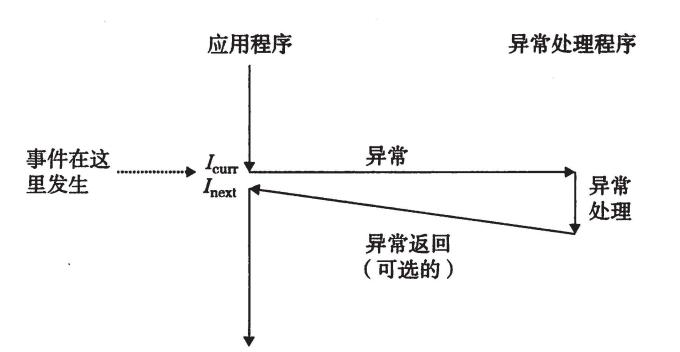
\includegraphics[width=15cm]{3-exception}
  \caption{异常处理图示}\label{fig:3-exception} 
\end{figure}

\subsection{异常的分发}

每当发生异常的时候,一般来说,处理器会进入一个用于分发异常的程序,
这个程序的作用就是检测发生了哪种异常,并调用相应的异常处理程序。
一般来说,这个程序会被要求放在固定的某个物理地址上(根据处理器的区别有所不同),
以保证处理器能在检测到异常时正确地跳转到那里。这个分发程序可以认为是操作系统的一部分。

代码\ref{code:exec_vec3}就是异常分发代码,
我们先将下面代码填充到我们的\mintinline{c}|start.S|的开头,然后我们来分析一下。

\label{code:exec_vec3}
\begin{minted}[linenos]{gas}
.section .text.exc_vec3
NESTED(except_vec3, 0, sp)
     .set noat
     .set noreorder
  1:
     mfc0 k1,CP0_CAUSE
     la   k0,exception_handlers
     andi k1,0x7c
     addu k0,k1
     lw   k0,(k0)
     NOP
     jr   k0
     nop
END(except_vec3)
     .set at
\end{minted}

\begin{exercise}
将异常分发代码填入 \textbf{boot/start.S} 合适的部分。
\end{exercise}

这段异常分发代码的作用流程简述如下:
\begin{enumerate}
  \item 取得异常码,这是区别不同异常的重要标志。
  \item 以得到的异常码作为索引去exception\_handlers数组中找到对应的中断处理函数,后文中会有涉及。
  \item 跳转到对应的中断处理函数中,从而响应了异常,并将异常交给了对应的异常处理函数去处理
\end{enumerate}

\begin{figure}[htbp]
  \centering
  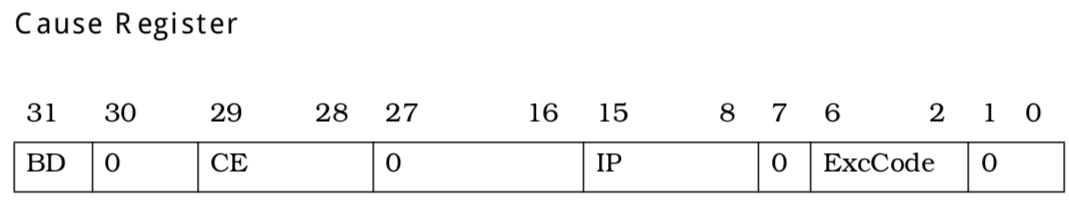
\includegraphics[width=15cm]{3-CauseRegister}
  \caption{CR寄存器}\label{fig:3-CauseRegister} 
\end{figure}
图\ref{fig:3-CauseRegister}是MIPS3000中Cause Register寄存器。
其中保存着CPU中哪一些中断或者异常已经发生。bit2~bit6保存着异常码,也就是根据异常码来识别具体哪一个异常发生了。
bit8~bit15保存着哪一些中断发生了。其他的一些位含义在此不涉及,可参看MIPS开发手册。

这个.text.exec\_vec3 段将通过链接器放到特定的位置,在R3000中要求是放到0x80000080地址处,
这个地址处存放的是异常处理程序的入口地址。一旦CPU发生异常,就会自动跳转到0x80000080地址处,
开始执行,下面我们将.text.exec\_vec3 放到该位置,一旦异常发生,就会引起该段代码的执行,
而该段代码就是一个分发处理异常的过程。

所以我们要在我们的lds中增加这么一段,从而可以让R3000出现异常时自动跳转到异常分发代码处。
\begin{minted}[linenos]{c}
. = 0x80000080;
.except_vec3 : {
    *(.text.exc_vec3)
}
\end{minted}


\begin{exercise}
将lds代码补全使得异常后可以跳到异常分发代码。
\end{exercise}


\subsection{异常向量组}
我们刚才提到了异常的分发,要寻找到exception\_handlers 数组中的中断处理函数,
而exception\_handlers 就是所谓的异常向量组。

下面我们跟随\mintinline{c}|trap_init(lib/traps.c)|函数来看一下,异常向量组里存放的是些什么?

\begin{minted}[linenos]{c}
extern void handle_int();
extern void handle_reserved();
extern void handle_tlb();
extern void handle_sys();
extern void handle_mod();
unsigned long exception_handlers[32];

void trap_init()
{
    int i;

    for (i = 0; i < 32; i++) {
        set_except_vector(i, handle_reserved);
    }

    set_except_vector(0, handle_int);
    set_except_vector(1, handle_mod);
    set_except_vector(2, handle_tlb);
    set_except_vector(3, handle_tlb);
    set_except_vector(8, handle_sys);
}
void *set_except_vector(int n, void *addr)
{
    unsigned long handler = (unsigned long)addr;
    unsigned long old_handler = exception_handlers[n];
    exception_handlers[n] = handler;
    return (void *)old_handler;
}

\end{minted}

实际上呢,这个函数实现了对全局变量exception\_handlers[32]数组初始化的工作,
其实就是把相应的处理函数的地址填到对应数组项中。
主要初始化
\begin{description}
  \item[0号异常]的处理函数为handle\_int,
  \item[1号异常]的处理函数为handle\_mod,
  \item[2号异常]的处理函数为handle\_tlb,
  \item[3号异常]的处理函数为handle\_tlb,
  \item[8号异常]的处理函数为handle\_sys,
\end{description}
一旦初始化结束,有异常产生,那么其对应的处理函数就会得到执行。而在我们的实验中,我们主要是
要使用0号异常,即中断异常的处理函数。因为我们接下来要做的,就是要产生时钟中断。

\subsection{时钟中断}

希望你还没有忘记在计组实验中所接触到的\textbf{定时器}这个概念。或许你当时对定时器的作用会有疑惑,
为了防止你继续迷糊不清,我们下面来简单介绍一下时钟中断的概念。

时钟中断和操作系统的时间片轮转算法是紧密相关的。时间片轮转调度是一种很公平的算法。
每个进程被分配一个时间段,称作它的时间片,即该进程允许运行的时间。如果在时间片结束时进程还在运行,
则该进程将挂起,切换到另一个进程运行。那么CPU是如何知晓一个进程的时间片结束的呢?就是通过定时器产生的时钟中断。
当时钟中断产生时,当前运行的进程被挂起,我们需要在调度队列中选取一个合适的进程运行。
如何“选取”,就要涉及到进程的调度了。

要产生时钟中断,我们不仅要了解中断的产生与处理。我们还要了解gxemul是如何模拟时钟中断的。
初始化时钟主要是在 kclock\_init 函数中,该函数主要调用set\_timer 函数,完成如下操作:
\begin{itemize}
  \item 首先向0xb5000100位置写入1,其中0xb5000000是模拟器(gxemul)映射实时钟的位置。偏移量为0x100表示来设置实时钟中断的频率,1则表示1秒钟中断1次,如果写入0,表示关闭实时钟。实时钟对于R3000来说绑定到了4号中断上,故这段代码其实主要用来触发了4号中断。注意这里的中断号和异常号是不一样的概念,我们实验的异常包括中断。
  \item 一旦实时钟中断产生,就会触发MIPS中断,从而MIPS将PC指向\mintinline{c}|0x80000080|,从而跳转到\mintinline{c}|.text.exc_vec3|代码段执行。对于实时钟引起的中断,通过text.exc\_vec3代码段的分发,最终会调用handle\_ int函数来处理实时钟中断。
  \item 在handle\_ int判断\mintinline{c}|CP0_CAUSE|寄存器是不是对应的4号中断位引发的中断,如果是,则执行中断服务函数timer\_ irq。
  \item 在timer\_ irq里直接跳转到sched\_ yield中执行。而这个函数就是我们将要补充的调度函数。
\end{itemize}

以上就是我们时钟中断的产生与中断处理流程,我们在这里要完成下面的任务以顺利产生时钟中断。

\begin{exercise}
通过上面的描述,补充 \textbf{ kclock\_init } 函数。
\end{exercise}

\subsection{进程调度}

通过上面的描述,我们知道了,其实在时钟中断产生时,最终是调用了sched\_ yield函数来进行进程的调度,
这个函数在\mintinline{c}|lib/sched.c|中所定义。这个函数就是我们本次最后要写的调度函数。
调度的算法很简单,就是时间片轮转的算法,没有优先级,根据注释就可以轻松写出。

\begin{exercise}
根据注释,完成 \textbf{sched\_yield }函数的补充。
\end{exercise}

至此,我们的实验三就算是圆满完成了。

\section{实验正确结果}
如果你按流程做下来并且做的结果正确的话,你运行之后应该会出现这样的结果

\begin{minted}[linenos]{text}
init.c: mips_init() is called

Physical memory: 65536K available, base = 65536K, extended = 0K

to memory 80401000 for struct page directory.

to memory 80431000 for struct Pages.

mips_vm_init:boot_pgdir is 80400000

pmap.c:  mips vm init success

panic at init.c:27: ^^^^^^^^^^^^^^^^^^^^^^^^^^^^^^^^^^^^^

2 2 2 2 2 2 2 2 2 2 2 2 2 2 2 2 2 2 2 2 2 2 2 2 2 2 2 2 2 
1 1 1 1 1 1 1 1 1 1 1 1 1 1 1 1 1 1 1 1 1 1 1 1 1 1 1 1   
2 2 2 2 2 2 2 2 2 2 2 2 2 2 2 2 2 2 2 2 2 2 2 2 2 2 2 
1 1 1 1 1 1 1 1 1 1 1 1 1 1 1 1 1 1 1 1 1 1 1 1 1 1 1 1 1 1 
2 2 2 2 2 2 2 2 2 2 2 2 2 2 2 2 2 2 2 2 2 2 2 2 2 2 2 2 2 
1 1 1 1 1 1 1 1 1 1 1 1 1 1 1 1 1 1 1 1 1 1 1 1 1 1 1 1 1 
\end{minted}

当然不会这么整齐,且没有换行,只是交替输出2和1而已~当然还不能放过你,你还需要再思考一部分内容

\begin{thinking}\label{think-调度}
思考一下你的调度程序,这种调度方式由于某种不可避免的缺陷而造成对进程的不公平。
  \begin{itemize}
    \item 这种不公平是如何产生的?
    \item 如果实验确定只运行两个进程,你如何改进可以降低这种不公平?
  \end{itemize}
\end{thinking}

\section{实验思考}

\begin{itemize}
\item \hyperref[think-env_init]{\textbf{\textcolor{baseB}{思考-init的逆序插入}}}
\item \hyperref[think-env_setup_vm]{\textbf{\textcolor{baseB}{思考-地址空间初始化}}}
\item \hyperref[think-user-data]{\textbf{\textcolor{baseB}{思考-user\_data的作用}}}
\item \hyperref[think-位置]{\textbf{\textcolor{baseB}{思考-位置的含义}}}
\item \hyperref[think-pc]{\textbf{\textcolor{baseB}{思考-进程上下文的PC值}}}
\item \hyperref[think-TIMESTACK]{\textbf{\textcolor{baseB}{思考-TIMESTACK的含义}}}
\item \hyperref[think-调度]{\textbf{\textcolor{baseB}{思考-不公的调度}}}
\end{itemize}

\section{挑战性任务}
我们实验中使用的调度算法是很简单的,那么现在希望你可以向内核中添加自己的调度策略,比如带优先级的时间片轮转算法。
修改调度算法,并利用测试的现象说明调度算法是正确的。如果你做了这部分的挑战性任务,请将代码提交到分支
\textbf{lab3-challenge}并推送到服务器上,并在实验文档中写入新的调度策略对于结果的影响并说明为什么,
可以自定义测试程序。
